\section{Support-projected one-step leakage of one global operator}
\label{app:global_k_support_closure}

This diagnostic tests a narrow mechanism hypothesis: a single learned global
operator can act approximately within several support-selected coordinate
sets on observed projected codes even when no basin label, basin count, or
trajectory-to-basin assignment is used.
It does not train local operators. In the implementation's row-vector
convention, a family mask defines a diagonal projector \(P_f\) and the learned
prediction is \(z_{t+1}=z_tK\). Cross-support output is therefore
\(z_tP_fK(I-P_f)\). This is the transpose-equivalent of
\((I-P_f)KP_fz_t\) in the paper's column-vector convention.

\paragraph{Existence construction.}
One matrix is not mathematically incompatible with several local laws. For
row-form affine dynamics $x^+=xA_b+c_b$, let
$\psi_b(x)=[x,1]$ and
$K_b=\left[\begin{smallmatrix}A_b&0\\c_b&1\end{smallmatrix}\right]$.
In an overcomplete direct-sum lift, set $K=\operatorname{diag}(K_1,\ldots,K_B)$
and let a routed basin-interior encoder place $\psi_b(x)$ only in block $b$. If $P_b$ selects that
block, then $P_bK(I-P_b)=0$ and $zP_bK^h=zK^h$, while different restrictions
contain different laws; a block-aware decoder recovers the physical state.
Unused blocks mean the architecture need not be told the realized basin count.
This proves an algebraic interior-chart possibility with a block-aware decoder,
not a continuous global encoder across basin boundaries, learned discovery,
label-free routing, or realization by our checkpoints.

\paragraph{Protocol frozen before evaluation.}
The roster contains unstructured signed sparse encoders with full
\(256\times256\) learned matrices: three initialization seeds on each of the
15 two-dimensional controlled systems. Their sign-split ReLU output
mechanically permits at most one active coefficient per positive/negative
pair, so the result concerns the learned sign-split coordinate basis rather
than generic sparse encoders. For every checkpoint, 128 newly generated trajectories
are split 64/64 by whole trajectory. The first half alone forms support
families using \(\lvert z_i\rvert>10^{-3}\), greedy Jaccard-0.50 merging, and a
minimum of 128 fit transitions per retained family. The second half alone is
scored. The primary slice contains transitions whose current and next support
masks both map to the same retained family. This future-conditioned
persistence criterion makes the closure test easier and is an important scope
restriction. The authenticated evaluator also emitted an all-current regime
before execution, without conditioning on the next support. Its reduction was
performed post hoc as a no-next-state guard and is not a second frozen
decision. Eligibility requires
at least two retained families, current/persistent coverage of at least
\(0.80/0.70\), and at least 64 scored transitions per reported family.

The activity leakage diagnostic is
\(\lVert zP_fK(I-P_f)\rVert/\lVert zP_fK\rVert\); its matrix-wide analogue is
\(\lVert P_fK(I-P_f)\rVert_F/\lVert P_fK\rVert_F\). To exclude the trivial case
where \(K\approx I\), change-normalized versions instead use
\(\lVert zP_f(K-I)\rVert\) and \(\lVert P_f(K-I)\rVert_F\) in their denominators.
We also report the inside-support residual of the
post-hoc restricted predictor \(P_fKP_f\), the encoded next-state energy
outside the current support, and the residual of the unmodified global \(K\)
relative to identity. The restricted predictor is an evaluation diagnostic,
not a retrained model. Finally, pairwise symmetric normalized Frobenius
distance between restricted operators tests whether the selected coordinate sets have
more differentiated restrictions than a matched null.

The null uses 16 coordinate permutations frozen in advance. Each permutation
moves positive/negative sign partners together and is applied jointly to
codes, next codes, masks, and projectors while leaving \(K\) fixed. It
therefore preserves norms, support cardinality, activity, and sign-split
semantics while breaking alignment with the learned operator. Metrics reduce
first within a run, then by the median across eligible seeds within each
system, and finally by the median across eligible systems; transitions are not
treated as independent replicates.

\begin{table}[tbp]
\centering
\caption{Held-out one-step support-closure diagnostics for one unchanged
global \(K\). The table reports both the post-hoc reduction of the
pre-execution evaluator-emitted all-current guard and the internally frozen
persistent-family primary. The matched null permutes sign pairs while holding
\(K\) fixed. The frozen branch is labeled partial closure, but its failed
differentiation guard permits only a lower-leakage claim.}
\label{tab:global_k_support_closure}
\resizebox{\textwidth}{!}{\begin{tabular}{llrrrrl}
\toprule
Slice & Diagnostic & Observed & Matched null & Obs./null & Wins & Gate \\
\midrule
All-current guard$^{\dagger}$ & Raw-$K$ activity leakage & 0.0047 & 0.2065 & 0.022 & 15/15 & Ref. pass \\
 & Raw-$K$ matrix Frobenius leakage & 0.0538 & 0.2080 & 0.240 & 15/15 & Diagnostic \\
 & $(K-I)$-normalized leakage & 0.3382 & 0.7830 & 0.433 & 15/15 & Ref. pass \\
 & $(K-I)$ matrix Frobenius leakage & 0.5541 & 0.7834 & 0.699 & 15/15 & Diagnostic \\
 & Post-hoc $PKP$ inside residual & 0.0100 & 0.1646 & 0.053 & 15/15 & Ref. pass \\
 & Restricted-operator distance & 0.9741 & 0.9830 & 0.993 & 0/15 & \textbf{Ref. fail} \\
\midrule
Persistent primary & Raw-$K$ activity leakage & 0.0047 & 0.2065 & 0.022 & 15/15 & Pass \\
 & Raw-$K$ matrix Frobenius leakage & 0.0538 & 0.2080 & 0.240 & 15/15 & Diagnostic \\
 & $(K-I)$-normalized leakage & 0.3394 & 0.7831 & 0.435 & 15/15 & Pass \\
 & $(K-I)$ matrix Frobenius leakage & 0.5539 & 0.7834 & 0.699 & 15/15 & Diagnostic \\
 & Post-hoc $PKP$ inside residual & 0.0100 & 0.1646 & 0.053 & 15/15 & Pass \\
 & Restricted-operator distance & 0.9741 & 0.9830 & 0.993 & -- & \textbf{Fail} \\
\midrule
\multicolumn{7}{l}{\footnotesize $^\dagger$Post-hoc reduction of a pre-execution evaluator-emitted no-next-state guard; not a second frozen decision.} \\
\multicolumn{7}{l}{\footnotesize The guard adds only 3,527 transitions (0.96 percentage points); medians are over system-level seed medians.} \\
\multicolumn{7}{l}{\footnotesize Frozen primary decision: partial closure; the differentiation guard fails; $PKP$ is a post-hoc restriction.} \\
\bottomrule
\end{tabular}
}
\end{table}

\begin{table}[tbp]
\centering
\caption{Triggered exact-dense specificity control. Dense tanh models use
zero weight decay and no sparsity-producing mechanism. At every matched
physical state, the dense projector selects the top-magnitude coordinates
with exactly the corresponding sparse support cardinality. Values are
observed/permutation-null ratios; the last column is sparse/dense. The
source-locked reducer retains 41/45 dense runs and 14 systems, versus 45/45
runs and 15 systems for sparse; its pre-outcome two-eligible-seed rule was
omitted from the card. Sparse-to-dense ratios of observed/null activity and
residual are 0.039/0.108 on the 14 common systems, 0.040/0.109 under the literal-card all-15 rule, and 0.041/0.110
when all three seeds are required (12 systems).}
\label{tab:global_k_dense_specificity}
\resizebox{0.82\textwidth}{!}{\begin{tabular}{lrrr}
\toprule
Metric & Sparse / null & Dense / null & Sparse / dense \\
\midrule
Raw-$K$ activity leakage / null & 0.022 & 0.567 & 0.039 \\
Post-hoc restricted residual / null & 0.053 & 0.486 & 0.108 \\
\bottomrule
\end{tabular}
}
\end{table}

\begin{figure*}[tbp]
\centering
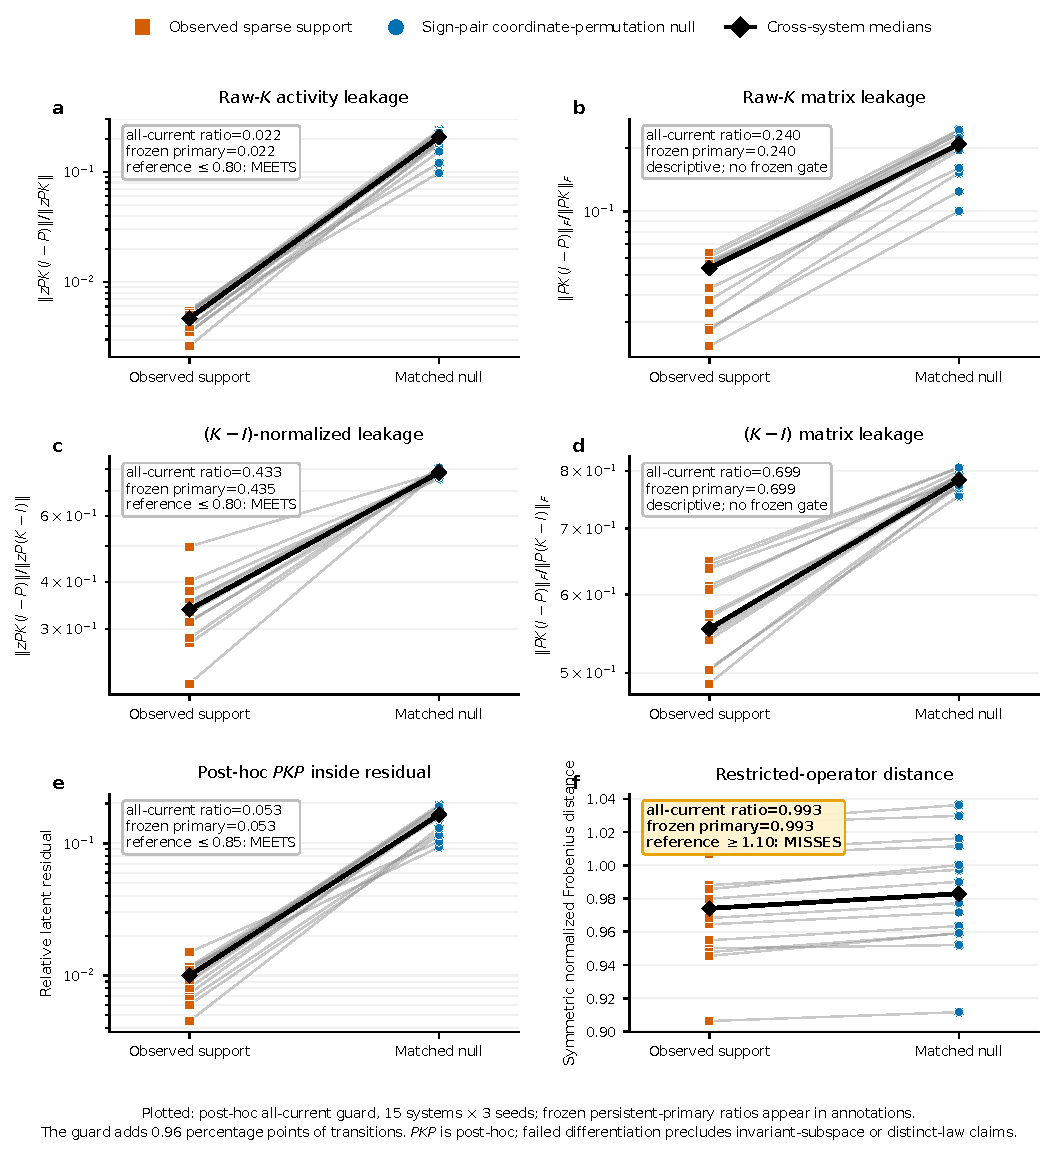
\includegraphics[width=\textwidth]{figures/neurips_paper_2026/global_k_support_closure_paired_systems.pdf}
\caption{System-level seed medians for the no-next-state all-current guard;
annotations give its ratio and the internally frozen persistent-primary ratio.
Lower is better in the first five panels. The two matrix-wide panels are
descriptive diagnostics without retrofitted decision thresholds.
Restricted-operator differentiation
is null-like and fails its reference threshold.}
\label{fig:global_k_support_closure}
\end{figure*}

All 45 runs and all 15 systems are eligible. Mean current and persistent
coverage are \(0.963\) and \(0.953\). Retained families average 5.84 per run,
their representatives average 95.0 of 256 coordinates, and the projected
source captures 0.997 of source-code RMS energy. At the system-median level,
the all-current observed/null activity leakage is \(0.0047/0.2065\) (ratio
\(0.022\)); change-normalized leakage is \(0.338/0.783\) (ratio \(0.433\));
the corresponding matrix-wide values are \(0.0538/0.2080\) (ratio \(0.240\))
and \(0.554/0.783\) (ratio \(0.699\)); and restricted inside-support residual
is \(0.0100/0.1646\) (ratio \(0.053\)). All 15 systems favor the observed masks
on each of these five diagnostics. Their ratios are numerically close to the
frozen persistent-primary values \(0.022/0.240/0.435/0.699/0.053\). Removing
the next-family condition therefore leaves the aggregate essentially
unchanged on this high-persistence sample. Because the guard adds only 3,527
transitions, or 0.96 percentage points, it does not determine behavior on
boundary-switching transitions. The unmodified
global-\(K\) residual is 0.583 times identity on the all-current guard.

The frozen strong decision nevertheless fails: restricted-operator distance
is \(0.974\) for observed supports and \(0.983\) under the null, a ratio of
\(0.993\) rather than the required \(1.10\). Thus support-projected one-step
leakage is lower than under matched permutations in this learned sign-split
basis, but the result does not establish distinct local laws, exact invariant subspaces, a direct-sum
decomposition, decoded forecasting, or Allen--Cahn behavior. Because the
result is basis-dependent, the frozen protocol triggered a
cardinality-matched exact-dense tanh specificity control.

That control is complete. Across the 45-run dense roster, 41 runs and 14
systems meet the source-locked reducer's eligibility rule. Sparse/dense
observed-to-null ratios are $0.039$ for raw-$K$ activity leakage and
$0.108$ for the post-hoc $P_fKP_f$ residual, far below both frozen $0.90$
gates; all 14 common eligible systems favor sparse on both metrics. The
reducer's requirement of at least two eligible seeds per system existed before
outcomes but was omitted from the prediction card, so it is not described as
card-preregistered; the frozen headline also aggregates 15 sparse versus 14
dense systems. Common-14 sensitivities are $0.039/0.108$, literal-card
minimum-one-seed all-15 sensitivities are $0.040/0.109$, and an all-three-seed
12-system sensitivity is $0.041/0.110$, so the conclusion is nearly unchanged
under these population choices. Thus the low support-projected one-step leakage
is specific to the complete sparse recipe relative to cardinality-matched
dense tanh top-$k$ coordinate masks. Dense masks have no natural dense-support semantics, and
encoder/decoder parameterization and optimization differ; this is a
complete-recipe specificity control, not a sparsity-only causal ablation,
basis-invariant result, distinct-law test, or forecasting comparison.

\paragraph{Prospective physical-law test.}
A separate frozen test trained ten new paired sparse/dense models on a
controlled two-dimensional system with three basin-specific laws. Training
and support-family discovery used neither basin labels nor the basin count;
evaluation labels only matched discovered families to the benchmark laws.
The authenticated result is negative. Only 24/30 sparse seed--basin rows
passed the prespecified differentiability gate, leaving 6/10 complete sparse
seeds rather than the required 8/10. On those rows, the Jacobian of the actual
restricted predictor selected the correct law in 9/24 nearest-law comparisons,
passed its ratio gate in 4/24, its affine gate in 2/24, and its finite-radius
gate in 0/24. The isolated $K$-induced update component was descriptively
nearest to the correct law in 24/24 rows and met projected-code closure in
23/24, but its aggregate matched-null guard failed (null won 6/10 seeds;
$p=0.377$). Dense specificity was invalid because only six pairs were jointly
differentiable. The isolated-component diagnostic is therefore stronger than
the actual-predictor diagnostic, but it also fails its aggregate null and the
packet fails validity. This contrast motivates testing reconstruction geometry
without identifying it as the cause and supports no multiple-law,
invariant-subspace, or sparse-superiority claim.

A final frozen recursive residual-routing diagnostic used one unchanged $K$
but did not yield a scientific decision: five of ten seed shards completed, a
sixth encountered a nonfinite payload value (\texttt{inf}) during strict serialization, four were
not run, and the required telemetry assessment and summary were absent. Under
its exact-ten fail-closed protocol, every forecasting claim tier is
invalid at the frozen validity tier and directionally unadjudicated; no partial
shard was inspected and the execution is not evidence for or against the hypothesis.
